
\section{Introduction to the logic analyzer}

The second part of the lab is to help you familiarize yourself with the logic analyzer. 

You should start by installing the logic analyzer software, as explained in Appendix~\ref{app:software_logic_analyzer}. You can connect the female-to-female cables to the logic analyzer inputs, and male-to-male pin headers at the end of each cable (feel free to detach the cables and to snap the male-to-male pin headers to the amount you prefer). 

In the following subsections, you will learn how to operate the logic analyzer: 
\begin{itemize}
	\item running the logic analyzer manually; 
	\item using the logic analyzer trigger. 
\end{itemize}
You can always refer to the logic analyzer tutorial (\url{https://learn.sparkfun.com/tutorials/using-the-usb-logic-analyzer-with-sigrok-pulseview}). 




\subsection{Running the logic analyzer manually}

We will use the logic analyzer to measure the execution time of parts of our code. The code needs to be instrumented to make internal signals from the microcontroller visible from the outside. 

\E{
\label{ex:4}
In this exercise, we will measure the period at which a GPIO is toggled. 
\begin{itemize}
	\item Using the \texttt{CyDelay} function, write a code to toggle the first GPIO on jumper J1 of the extension board at a frequency of 20~Hz. There is no need to use a hardware timer for this exercise; 
	\item Connect the analyzer to the extension board as shown in Figure~\ref{fig:analyserConnection}. 
	\item Use the \texttt{PulseView} software to measure the period with which the GPIO is toggled. 
\end{itemize}
}
{}

\begin{figure}[h]
	\centering
	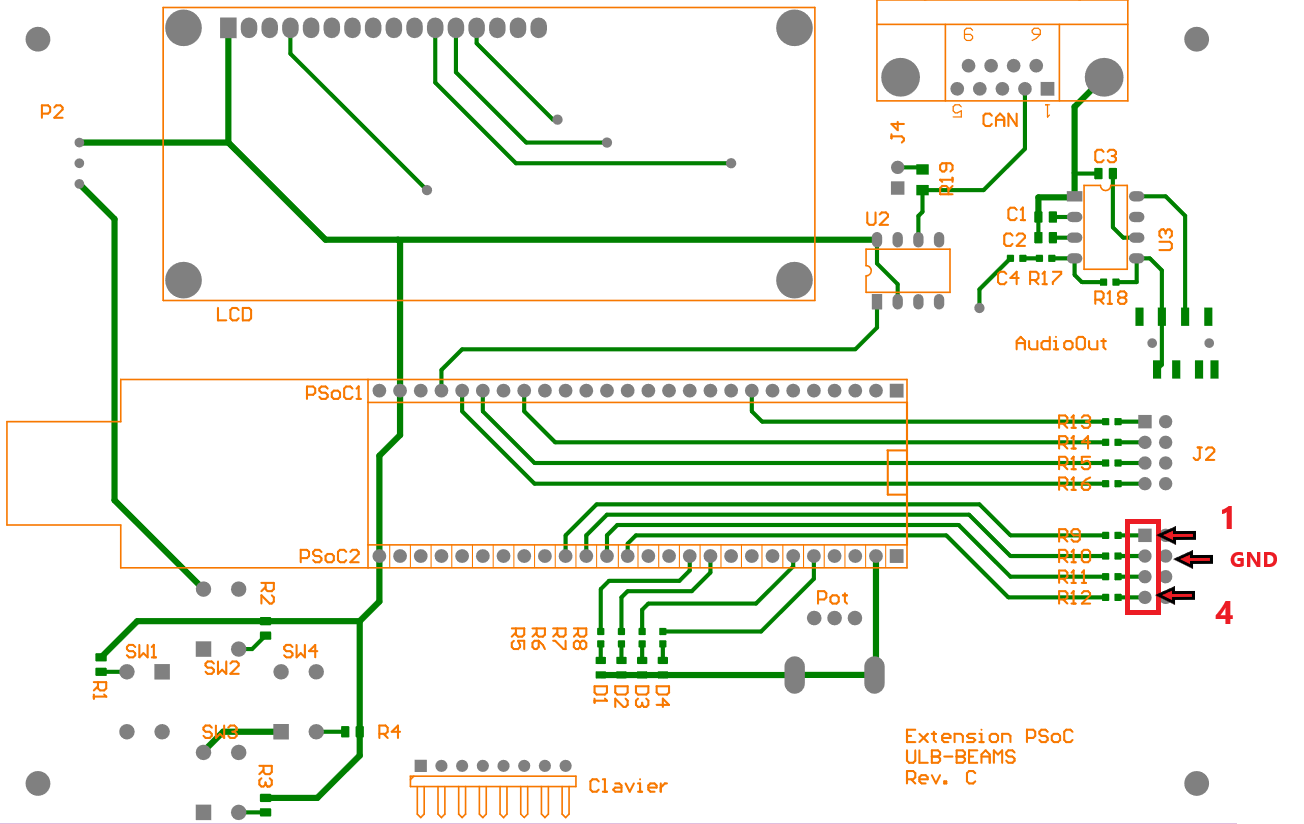
\includegraphics[width=4in]{analyserConnection.png}
	\caption{Where to connect the logic analyzer to the extension board. }
	\label{fig:analyserConnection}
\end{figure}




\subsection{Using the logic analyzer trigger}

A trigger can be used to automate the acquisition of the logic analyzer. You can select a trigger by selecting the channel to trigger on (e.g. D3) and selecting the required trigger (e.g. rising edge). 

It is also possible to trigger the acquisition based on multiple channels, you just need to specify the trigger condition for each channel (e.g. trigger when D1 is high and D2 has a rising edge). 

\E{
\label{ex:5}
In this exercise, we will trigger the logic analyzer when SW4 is pressed. 
\begin{itemize}
	\item Extend your previous code such that the second GPIO of jumper J1 becomes high when SW4 is pressed, and becomes low when SW4 is released; 
	\item Specify a trigger condition such that the logic analyzer acquisition is triggered when SW4 is pressed. 
	\item Extend your previous code and trigger conditions such that the acquisition is triggered when SW3 is high and SW4 is pressed. 
\end{itemize}
}
{}









